\PassOptionsToPackage{unicode=true}{hyperref} % options for packages loaded elsewhere
\PassOptionsToPackage{hyphens}{url}
%
\documentclass[ignorenonframetext,]{beamer}
\usepackage{pgfpages}
\setbeamertemplate{caption}[numbered]
\setbeamertemplate{caption label separator}{: }
\setbeamercolor{caption name}{fg=normal text.fg}
\beamertemplatenavigationsymbolsempty
\usepackage{lmodern}
\usepackage{amssymb,amsmath}
\usepackage{ifxetex,ifluatex}
\usepackage{fixltx2e} % provides \textsubscript
\ifnum 0\ifxetex 1\fi\ifluatex 1\fi=0 % if pdftex
  \usepackage[T1]{fontenc}
  \usepackage[utf8]{inputenc}
  \usepackage{textcomp} % provides euro and other symbols
\else % if luatex or xelatex
  \usepackage{unicode-math}
  \defaultfontfeatures{Ligatures=TeX,Scale=MatchLowercase}
\fi
\usecolortheme{beaver}
\usefonttheme{professionalfonts}
% use upquote if available, for straight quotes in verbatim environments
\IfFileExists{upquote.sty}{\usepackage{upquote}}{}
% use microtype if available
\IfFileExists{microtype.sty}{%
\usepackage[]{microtype}
\UseMicrotypeSet[protrusion]{basicmath} % disable protrusion for tt fonts
}{}
\IfFileExists{parskip.sty}{%
\usepackage{parskip}
}{% else
\setlength{\parindent}{0pt}
\setlength{\parskip}{6pt plus 2pt minus 1pt}
}
\usepackage{hyperref}
\hypersetup{
            pdftitle={Einleitung und Motivation},
            pdfauthor={Jan-Philipp Kolb},
            pdfborder={0 0 0},
            breaklinks=true}
\urlstyle{same}  % don't use monospace font for urls
\newif\ifbibliography
\usepackage{graphicx,grffile}
\makeatletter
\def\maxwidth{\ifdim\Gin@nat@width>\linewidth\linewidth\else\Gin@nat@width\fi}
\def\maxheight{\ifdim\Gin@nat@height>\textheight\textheight\else\Gin@nat@height\fi}
\makeatother
% Scale images if necessary, so that they will not overflow the page
% margins by default, and it is still possible to overwrite the defaults
% using explicit options in \includegraphics[width, height, ...]{}
\setkeys{Gin}{width=\maxwidth,height=\maxheight,keepaspectratio}
% Prevent slide breaks in the middle of a paragraph:
\widowpenalties 1 10000
\raggedbottom
\setbeamertemplate{part page}{
\centering
\begin{beamercolorbox}[sep=16pt,center]{part title}
  \usebeamerfont{part title}\insertpart\par
\end{beamercolorbox}
}
\setbeamertemplate{section page}{
\centering
\begin{beamercolorbox}[sep=12pt,center]{part title}
  \usebeamerfont{section title}\insertsection\par
\end{beamercolorbox}
}
\setbeamertemplate{subsection page}{
\centering
\begin{beamercolorbox}[sep=8pt,center]{part title}
  \usebeamerfont{subsection title}\insertsubsection\par
\end{beamercolorbox}
}
\AtBeginPart{
  \frame{\partpage}
}
\AtBeginSection{
  \ifbibliography
  \else
    \frame{\sectionpage}
  \fi
}
\AtBeginSubsection{
  \frame{\subsectionpage}
}
\setlength{\emergencystretch}{3em}  % prevent overfull lines
\providecommand{\tightlist}{%
  \setlength{\itemsep}{0pt}\setlength{\parskip}{0pt}}
\setcounter{secnumdepth}{0}

% set default figure placement to htbp
\makeatletter
\def\fps@figure{htbp}
\makeatother


\title{Einleitung und Motivation}
\author{Jan-Philipp Kolb}
\date{22 Oktober 2018}

\begin{document}
\frame{\titlepage}

\begin{frame}{Start}
\protect\hypertarget{start}{}

\url{http://rpubs.com/Japhilko82/gesis_mannheim}

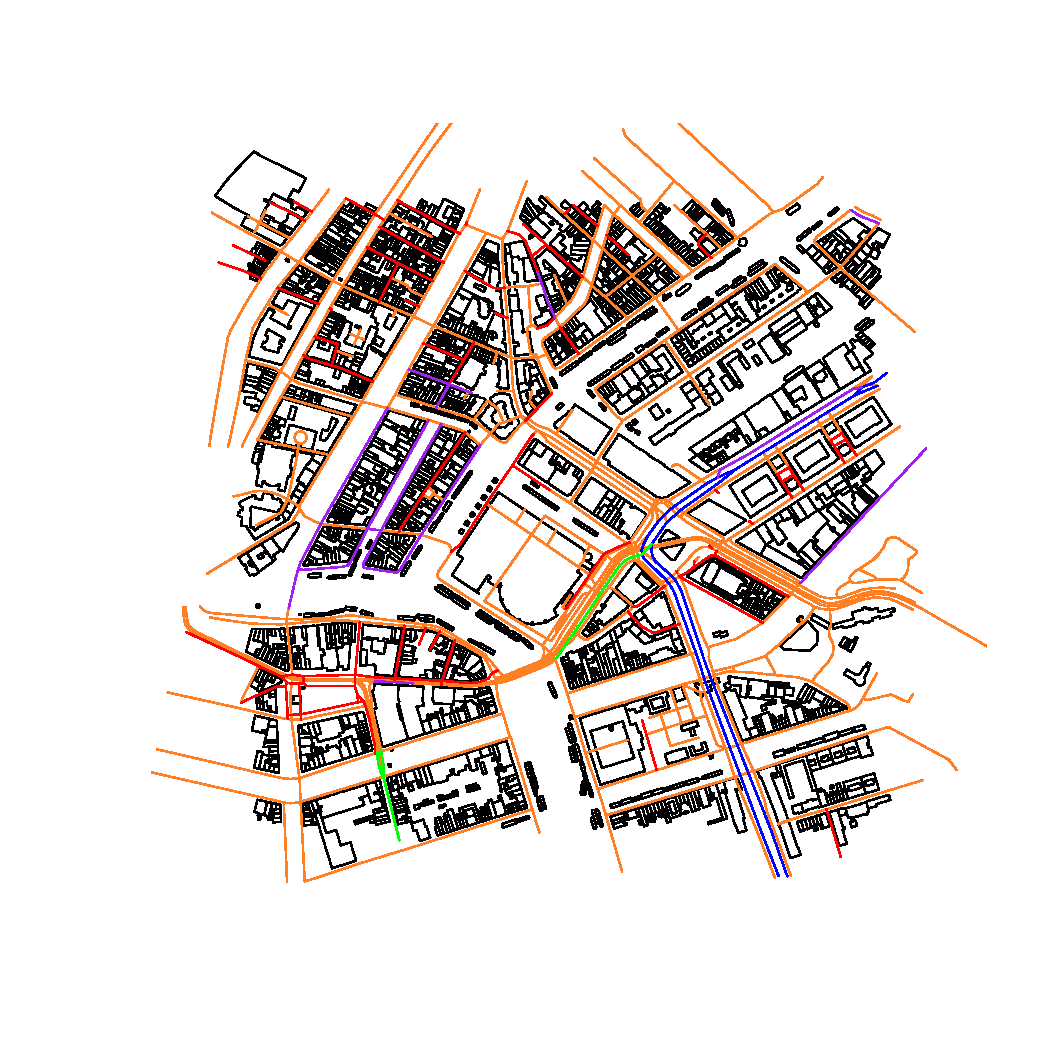
\includegraphics{figure/Amsterdam_osmplotr_highways.pdf}

\end{frame}

\begin{frame}{Outline}
\protect\hypertarget{outline}{}

\begin{itemize}
\tightlist
\item
  Spatial Turn - why this course
\item
  Research questions
\item
  Available data
\item
  Neogeograpy
\item
  Realisation
\end{itemize}

\end{frame}

\begin{frame}{\href{http://de.slideshare.net/rheimann04/big-social-data-the-spatial-turn-in-big-data}{Laws
of Spatial Sience}}
\protect\hypertarget{laws-of-spatial-sience}{}

\href{https://en.wikipedia.org/wiki/Tobler's_first_law_of_geography}{Tobler's
law}

\begin{quote}
everything is related to everything else, but near things are more
related than distant things.
\end{quote}

\end{frame}

\begin{frame}{\href{https://de.wikipedia.org/wiki/Spatial_turn}{Spatial
Turn}}
\protect\hypertarget{spatial-turn}{}

\begin{quote}
Spatial turn is a term used to describe an intellectual movement that
places emphasis on place and space in social science and the humanities.
\end{quote}

\href{https://en.wikipedia.org/wiki/Spatial_turn}{Englisches Wikipedia}

\end{frame}

\begin{frame}{Regional/geographical differences in the perception
of\ldots{}}
\protect\hypertarget{regionalgeographical-differences-in-the-perception-of}{}

\begin{itemize}
\tightlist
\item
  \ldots{} measures to promote climatic change
\item
  \ldots{} big infrastructure projects
\end{itemize}

\end{frame}

\begin{frame}{Availability of data - Example Census Atlas}
\protect\hypertarget{availability-of-data---example-census-atlas}{}

\url{https://atlas.zensus2011.de/}
\includegraphics{https://raw.githubusercontent.com/Japhilko/GeoData/master/data/figure/Zensus_Mannheim2.png}

\end{frame}

\begin{frame}{Verfügbarkeit der Daten - Beispiel
\href{http://michael-hoerz.de/maps/berlin-bike/}{Fahrradunfälle in
Berlin}}
\protect\hypertarget{verfugbarkeit-der-daten---beispiel-fahrradunfalle-in-berlin}{}

\url{http://www.sowirdberlin.de/}
\includegraphics{https://asset0.torial.com/system/portfolio_item_images/production/2014/07/21/m5we1vmq6_preview_image_9678.jpg}

\end{frame}

\begin{frame}{Heterogener Datenbestand - Beispiel
\url{http://names.mappinglondon.co.uk/}}
\protect\hypertarget{heterogener-datenbestand---beispiel-httpnames.mappinglondon.co.uk}{}

\includegraphics{http://mappinglondon.co.uk/wp-content/uploads/2011/11/surnames1.png}

\end{frame}

\begin{frame}{Motivation - Warum die Darstellung in Karten}
\protect\hypertarget{motivation---warum-die-darstellung-in-karten}{}

\begin{itemize}
\item
  Darstellung in Karten ermöglicht besseres Verständnis bspw.
  sozialwissenschaftlicher Phänomene.
\item
  Attraktiver Output
\item
  Durch die INSPIRE Richtlinie und \emph{Collaborative Mapping} wächst
  der verfügbare Bestand an Geodaten.
\item
  Daten sind oft frei verfügbar im Internet (z.B. durch die Nutzung von
  APIs)
\item
  Die Daten sind allerdings oft wenig oder gar nicht strukturiert (z.B.
  Internet Dokumente), heterogen und
\item
  meistens nicht für die Nutzung zur räumlichen Visualisierung
  vorgesehen, beinhalten aber implizit geographische Informationen (Web
  2.0)
\item
  Oftmals sind wenig oder keine Metadaten vorhanden
\end{itemize}

\end{frame}

\begin{frame}{Übersicht - \href{http://www.edureka.co/}{warum R}}
\protect\hypertarget{ubersicht---warum-r}{}

\includegraphics{http://d287f0h5fel5hu.cloudfront.net/blog/wp-content/uploads/2013/06/bar-learn-r-img11.png}

\end{frame}

\begin{frame}{\href{http://blog.revolutionanalytics.com/}{R Nutzer rund
um die Welt}}
\protect\hypertarget{r-nutzer-rund-um-die-welt}{}

\includegraphics{http://revolution-computing.typepad.com/.a/6a010534b1db25970b0191035099d8970c-pi}

\end{frame}

\begin{frame}{\href{http://spatial.ly/}{Wo sind die aktivsten Nutzer?}}
\protect\hypertarget{wo-sind-die-aktivsten-nutzer}{}

\includegraphics{http://spatial.ly/wp-content/uploads/2013/06/r_activity.png}

\end{frame}

\begin{frame}{Was ist das Ziel - Straßen in Berlin}
\protect\hypertarget{was-ist-das-ziel---straen-in-berlin}{}

Dargestellt werden OpenStreetMap Daten, die mit der Overpass API
heruntergeladen wurden.

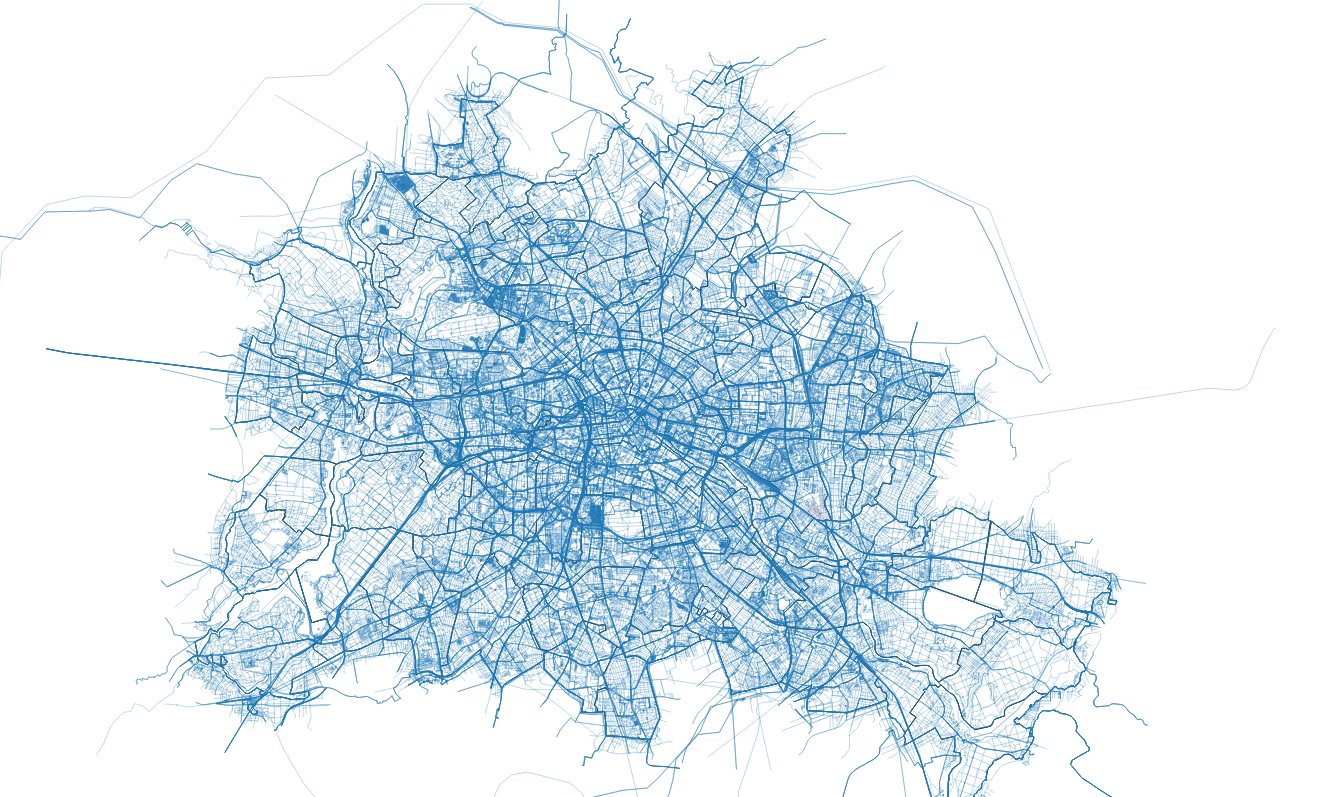
\includegraphics{https://raw.githubusercontent.com/Japhilko/GeoData/master/data/figure/streets_Berlin2.png}

\end{frame}

\begin{frame}{Links mit Beispielen}
\protect\hypertarget{links-mit-beispielen}{}

\begin{itemize}
\item
  Shiny App zu
  \href{https://japhilko.shinyapps.io/Choropleths/}{Indikatoren} für
  Europa
\item
  Räumliche Visualisierung in den USA -
  \href{https://rpubs.com/Radcliffe/walmart}{Walmarts in den USA}
\item
  \href{http://www.nytimes.com/interactive/2014/09/03/us/the-race-gap-in-americas-police-departments.html?_r=0}{Race
  Gap Police USA} - \href{http://fivethirtyeight.com/}{Wahl USA}
\item
  Zeit Artikel zum Zustand der
  \href{http://detektor.fm/digital/datenjournalismus-interaktive-karte-zeigt-marode-deutsche-bahn-bruecken}{Eisenbahnbrücken}
\item
  \href{http://michael-hoerz.de/maps/berlin-bike/}{Fahrradunfälle} in
  Berlin
\item
  \href{http://interaktiv.morgenpost.de/beta-fussballkarte/\#7/51.258/10.756}{Verteilung
  Fußballfans}
\item
  \href{http://news.nationalgeographic.com/news/2014/07/140715-ocean-plastic-debris-trash-pacific-garbage-patch/}{Plastiktüten
  im Meer}
\end{itemize}

Datenquellen:

\begin{itemize}
\tightlist
\item
  \href{https://www.pegelonline.wsv.de/gast/start}{Pegelstände} in
  Deutschland
\item
  \href{http://driven-by-data.net/}{driven by data}
\end{itemize}

Resourcen

\begin{itemize}
\tightlist
\item
  Andreas Plank -
  \href{http://www.chironomidaeproject.com/fileadmin/downloads/Formeln_in_R.pdf}{Grafiken
  und Statistik in R}
\end{itemize}

\end{frame}

\end{document}
